\documentclass{article}

\usepackage{tikz}
\usepackage{color}
\usetikzlibrary{fit,shapes,positioning,backgrounds,calc,patterns,scopes,decorations,chains,arrows}

\thispagestyle{empty}

\tikzset{fn-inact/.style={
    rectangle, fill=black!20, thick, draw=black,
    rounded corners=1ex,minimum height=2.5cm, minimum width=1.8cm
}}

\tikzset{fn-activ/.style={
    rectangle, fill=green!30, thick, draw=black,
    rounded corners=1ex,minimum height=2.5cm, minimum width=1.8cm
}}

\setlength{\parskip}{0pt}

\newenvironment{sItemize}{
  \begin{list}{-}{\leftmargin=1em\itemsep=0em\parskip=0pt\parsep=0pt}
}{\end{list}}

\definecolor{lightblue}{rgb}{0.68,0.85,0.90}
\definecolor{red3}{rgb}{0.80,0.00,0.00}
\definecolor{purple}{rgb}{0.63,0.13,0.94}



\begin{document}
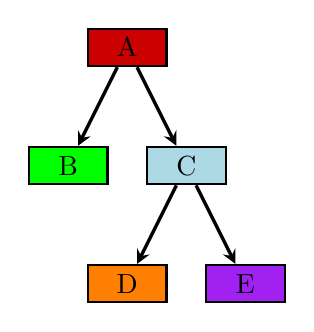
\begin{tikzpicture}
[every node/.style={minimum width=1cm, rectangle,draw,thick}, edge from parent/.style={draw,-stealth,very thick}]
\node[fill=red3] {A}
    child { node[fill=green] {B} }
    child { node[fill=lightblue] {C}
        child { node[fill=orange] {D} }
        child { node[fill=purple] {E} }
    };
\end{tikzpicture}
\end{document}
